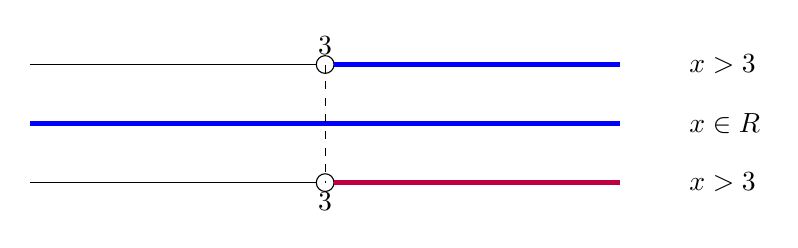
\begin{tikzpicture}[scale=0.75]
            %\draw (-11,0)-- (3,0); %AXIS
            %\foreach \x in {-1} {
            %    \draw (\x,0.5) -- (\x,-0.5) node[below] {$\x$};
            %}
            \draw (-2,1) -- (8,1);
            \draw[fill=white] (3,1) circle (0.15) node[above]{3};
            \node[anchor=west, right] at (9,1) {$x > 3$};
            \draw (-2,0) -- (8,0);
            \node[anchor=west, right] at (9,0) {$x \in \mathbb{R}$};
            \draw (-2,-1) -- (8,-1);
            \draw[fill=white] (3,-1) circle (0.15) node[below]{3};
            \draw[ultra thick, blue] (3.15,1) -- (8,1);
            \draw[ultra thick, blue] (-2,0) -- (8,0);
            \draw[ultra thick, purple] (3.15,-1) -- (8,-1);
            \node[anchor=west, right] at (9,-1) {$x > 3$};
            \draw[dashed] (3,1) -- (3,-1);
\end{tikzpicture}